\chapter{Literature Notes and Commentary}

\section{Reinforcement Learning Overview}

The reader may not be readily familiar with reinforcement learning (RL).
Thus, we here provide a brief overview of the terminology, basic definition, essential results, and common algorithms in RL theory.

\subsection{Markov Decision Process}

A Markov Decision Process (MDP) problem is a framework for modeling sequential decision-making by an agent in an environment.
A problem is formally defined as a $4$-tuple $(S, A, T, R)$.
\begin{itemize}
  \item $S$ is the state space, which is the set of all possible states of the environment.
  \item $A$ is the action space, which contains all possible actions that the agent can take (across all possible states).
  \item $T: S \times A \times S \to [0, 1]$ is the transition function in a stochastic environment. When the environment is in state $s$ and
    the agent takes action $a$, then $T(s, a, s')$ is the probability that the environment transitions to state $s'$ as a result. (In a deterministic environment,
    this function may not be necessary, as there may be only one possible state due to the taken action.)
  \item $R: S \times A \times S \to \R$ is the reward function. When the environment changes state from $s$ to $s'$ due to action $a$, the agent recieves reward $R(s, a, s')$.
\end{itemize}
The environment is Markov, which means that the distribution of the next state $s'$ conditioned on the current state $s$ and action $a$ is independent from the time step.

A policy is a function $\pi: S \to A$ that dictates actions to take at a given state.
A solution to an MDP problem is an optimal policy $\pi^*$ that maximizes the agent's utility, however that is defined.

\subsection{RL Terminology}

In RL, the agent's utility is generally defined as the total expected discounted reward.
Let $\gamma \in [0, 1]$ be a constant discount factor. The utility from a sequence of reward $\{r_t\}_{t=0}^\infty$ is
thus commonly defined as $U([r_0, r_1, \ldots]) = \sum_{t=0}^\infty \gamma^t r_t \leq \frac{\sup_t r_t}{1-\gamma}$.
The benefit of this formulation is that (1) utility is bounded if the rewards are bounded, and (2) there is a balance
between small immediate rewards and large long-term rewards. (The use of the discount factor depends on the actual reward function.
For custom reward functions, it may not be necessary or even desireable; we include it because it is common in RL literature.)

Given a policy $\pi: S \to A$, we define the value function $V^\pi: S \to \R$ and the $Q$-function $Q^\pi: S \times A \to \R$ as
\begin{align*}
  V^\pi(s) = \E_\pi\left[ \sum_{t=0}^\infty \gamma^t R_t \:\Big|\: s_0 = s  \right] &&
  Q^\pi(s, a) = \E_\pi\left[  \sum_{t=0}^\infty \gamma^t R_t \:\Big|\: s_0 = s, a_0 = a \right]
\end{align*}
$V^\pi(s)$ is the expected utility from starting at $s$ and following policy $\pi$, and $Q^\pi(s, a)$ is the expected utility
from starting at $s$, taking action $a$, and then following policy $\pi$ thereafter.
The goal of RL is to find the optimal policy $\pi^*$, from which we have the optimal value function $V^*$ and optimal $Q$-function $Q^*$.
These optimal values can further be defined as follows:
\begin{align*}
  Q^*(s, a) &= \E_{s'}[R(s, a, s') + \gamma V^*(s')] = \sum_{s'} T(s, a, s')[R(s, a, s') + \gamma V^*(s')] \\
  V^*(s) &= \max_a Q^*(s, a) = \max_a \sum_{s'} T(s, a, s')[R(s, a, s') + \gamma V^*(s')]
\end{align*}
The second equation is known as the Bellman equation.

There are two main branches of RL: model-based and model-free.
In model-based RL, the agent attempt to build a model of the environment transition function $T$ and reward function $R$.
Based on these model, it then attempts to directly maximize the total expected reward.
In model-free RL, the agent does not attempt to model the environment, but instead attempts to learn either the value function or $Q$-function.
Once it has one of these, it can derive an optimal policy from it as:
\begin{align*}
  \pi^*(s) = \arg\max_a Q^*(s, a) = \arg\max_a \sum_{s'} T(s, a, s')\left[ R(s, a) + \gamma V^*(s')\right]
\end{align*}
We proceed with model-free RL in this project.

\subsection{Specialization to Our Application}

In the portfolio optimization setting, our RL agent seeks to produce an optimal set of portfolio weights given all the information it knows.
Assume that there are $n$ tradeable stocks in our universe, and one risk-free asset.
The action space $A = \left\{a \in \R^{n+1} \:|\: \sum_i a_i = 1\right\}$ is the set of all possible portfolio weights.

The state space $S$ encompasses all information available to the agent when it is asked to make a portfolio allocation decision at a given time.
Depending on what information is provided, this could include past performance of the strategy, historical stock prices, encoded news information for
select/all tickers in the universe, or some combination of these. For most of the scenarios we consider, $S \in \R^{n \times N}$ is a matrix, where
each row corresponds to a different stock ticker, and along that row we find the past few weeks of historical price data as well as some
aggregate of news sentiment indicators/scores.

The transition function $T$ is a delta function since state transitions are deterministic.
The environment uses the weights provided by the agent to reallocate the portfolio, computes the new portfolio value,
and reads in new historical stock data and news datapoints to form the next state (for the next time period) which is provided to the agent.
(The exact for of $T$ is not needed; it is implicitly defined by the deterministic environment udpates.)

The reward function $R$ should be such that it encourages the agent to produce good portfolio weights.
One simple reward function is pure profit: $R(s_t, a_t)$ is how much profit is gained to portfolio allocation $a_t$ during time interval $[t, t+1)$.
Another possible reward function is the Differential Sharpe ratio (as described in section \ref{diff_sharpe_ratio_section}), which urges the agent to make portfolio allocations to maximize its total Sharpe ratio. 



\section{Differential Sharpe Ratio}
\label{diff_sharpe_ratio_section}

\cite{drl_mvo} utilizes the Differential Sharpe Ratio to implement and evaluate a reinforcement learning agent.
The Differential Sharpe Ratio is based on Portfolio Management Theory, and is developed in the author' previous works \cite{diff_sharpe_ratio_paper} and \cite{diff_sharpe_ratio_book}.
We briefly review the theory developed in both sources.

The traditional definition of the Sharpe Ratio is the ratio of expected excess returns to volatility.
If $R_t$ is the return of the portfolio at time $t$, and $r_f$ is the risk-free rate then
\begin{align*}
  \mathcal{S} = \frac{\mathbb{E}_t[R_t] - r_f}{\sqrt{\Var_t[R_t]}}
\end{align*}

This works well to analyze a strategy once all data is collected.
The goal of traditional portfolio theory is to maximize the Sharpe Ratio over the given time period (equivalently,
to maximize the mean-variance utility function).

Unfortunately, this will not work for a reinforcement learning agent. The agent must be given a reward after every time step,
but the traditional Sharpe ratio is only calculated at the end.

The Differential Sharpe Ratio attempts to remedy this by approximating a change in the total Sharpe ratio up to that point.
By summing together many of these incremental changes (though approximate), the cumulative rewards is an approximation of the total
Sharpe ratio over the complete time period.

The approximation works by updating moment-based estimators of the expectation and variance in the Sharpe Ratio formula.
Let $A_t$ and $B_t$ be estimates of the first and second moments of the return $R_t$ up to time $t$.
After time step $t$, having obtained $R_t$, we perform the following updates:
\begin{align*}
  \Delta A_t = R_t - A_{t-1} && A_t = A_{t-1} + \eta \Delta A_t \\
  \Delta B_t = R_t - B_{t-1} && B_t = B_{t-1} + \eta \Delta B_t
\end{align*}
where $A_0 = B_0 = 0$ and $\eta \sim 1/T$ is an update parameter, where there are $T$ total time periods.
These updates are essentially exponential moving averages.

Let $S_t$ be an approximation of the Sharpe Ratio up to time $t$ based on estimates $A$ and $B$. That is,
\begin{align*}
  S_t = \frac{A_t}{\sqrt{B_t - A_t^2}}
\end{align*}
The definition here ignores the risk-free rate term. $K_\eta$ is a normalization constant to ensure an unbiased estimator.

Pretend that at the update for time $t$, $A_{t-1}$ and $B_{t-1}$ are constants,
and $R_t$ is also a known constant. Then the updates to $A_t$ and $B_t$ really only depend on the time step parameter $\eta$.
Indeed, if $\eta = 0$, then $A_t = A_{t-1}$ and $B_t = B_{t-1}$, so $S_t = S_{t-1}$.
Now consider varying $\eta$; expanding the Sharpe ratio estimator formula in Taylor series gives
\begin{align*}
  S_t \approx S_{t-1} + \eta \frac{\diff S_t}{\diff \eta}\Big|_{\eta = 0} + o(\eta^2)
\end{align*}

If $\eta$ is small, the final term is negligible, so this formula gives us an exponential-moving-average update for $S_t$.
The Differential Sharpe Ratio is defined to be proportional derivative in that expression. With some tedious calculus, we find that
\begin{align*}
  D_t &= \frac{\diff S_t}{\diff \eta} = \frac{\diff}{\diff\eta}\left[ \frac{A_t}{\sqrt{B_t - A_t^2}} \right] = \frac{\frac{\diff A_t}{\diff \eta} \sqrt{B_t - A_t^2} - A_t \frac{\frac{\diff B_t}{\diff \eta} - 2 A_t \frac{\diff A_t}{\diff \eta}}{2 \sqrt{B_t - A_t^2}}}{B_t - A_t^2} \\
  &= \frac{\Delta A_t \sqrt{B_t - A_t^2} - A_t \frac{\Delta B_t - 2 A_t \Delta A_t}{2 \sqrt{B_t - A_t^2}}}{B_t - A_t^2}
  = \frac{B_t \Delta A_t - \frac{1}{2} A_t \Delta B_t}{(B_t - A_t^2)^{3/2}}
\end{align*}

This reward function is simple to implement in an environment. The authors of the original papers provide
experimental support for the value of this reward function in a reinforcement learning setting.




\section{Transaction Costs}
\label{transaction_costs_section}

\cite{drl_framework} contains an excellent walkthrough of the mathematics for modeling transaction costs
in RL environment updates. We provide a shortened version here.

Suppose we have $m$ tradeable assets and the risk-free asset. Let $\mathbf v_t = (1, v_{1,t}, v_{2,t}, \ldots v_{m,t}) \in \R^{m+1}$ be the
prices of the assets at time $t$ (the first entry is the risk-free asset). The raw return vector is defined as
$\mathbf y_t = \mathbf v_t \varoslash \mathbf v_{t-1} \in \R^{m+1}$, where division is element-wise. Suppose the portfolio
weight vector during time period $t$ is $\mathbf w_t \in \R^{m+1}$, and let the value of the portfolio value at time $t$ be $p_t$.
If we were not considering transaction costs, then the portfolio return would be $\frac{p_t}{p_{t-1}} = \mathbf y_t \cdot \mathbf w_t$.

Unfortunately, buying and selling assets incurs transaction costs. Let $\mathbf w_t' \in \R^{m+1}$ be the effective portfoliio weights
at the end of time $t$ (it has changed from $\mathbf w_t$ due to the changes in price). We have
\begin{align*}
  \mathbf w_t' = \frac{\mathbf y_t \odot \mathbf w_t}{\mathbf y_t \cdot \mathbf w_t}
\end{align*}
where $\odot$ is element-wise multiplication. Between time $t-1$ and time $t$, the portfolio value is also
adjusted from $p_{t-1} \in \R$ to $p_t' = p_{t-1} \mathbf y_t \cdot \mathbf w_{t-1}$. Let $p_t$ be the value of the portfolio
after transaction costs, and let $\mu_t \in \R$ be the transaction cost factor, such that $p_t = \mu_t p_t'$.
We can keep track of the relevant time of each variable with the following diagram:

\begin{center}
  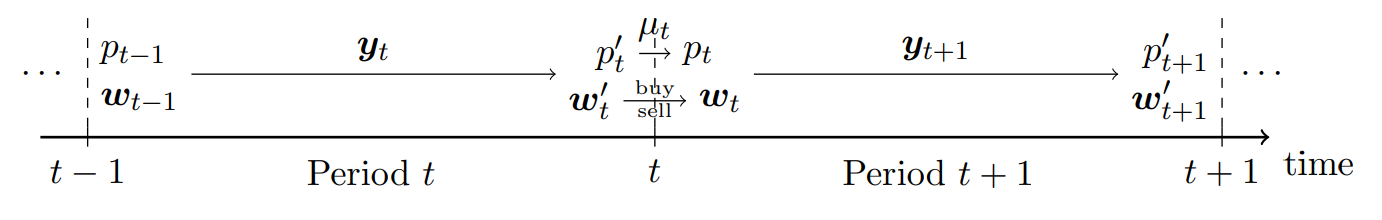
\includegraphics[width=13cm]{transaction_cost_time_updates.png}
\end{center}

In this paradigm, the final portfolio value at time $T$ is
\begin{align*}
  p_T = p_0 \prod_{t=1}^T \frac{p_t}{p_{t-1}} = p_0 \prod_{t=1}^T \mu_t \mathbf y_t \cdot \mathbf w_{t-1}
\end{align*}
The main difficulty is in determining the factor $\mu_t$, since it is an aggregate of all the transaction cost penalties.

Let $c_s \in [0, 1)$ be the commission rate for selling. We need to sell some amount of asset $i$ if 
there is more of asset $i$ in $\mathbf w_t'$ than in $\mathbf w_t$ by dollar value. Mathematically, this condition
is $p_t' w_{i,t}' > p_t w_{t,i}$, which is equivalent to $w_{i,t}' > \mu_t w_{i,t}$. Thus, the total amount of
money raised from selling assets is
\begin{align*}
  (1-c_s) p_t' \sum_{i=1}^m (w_{i,t}' - \mu_t w_{i,t})^+
\end{align*}
where $(\cdot)^+ = \max\{0, \cdot\} = \mathrm{ReLU}(\cdot)$. This money, as well as the money from adjusting the cash reserve
from $p_t' w_{0,t}'$ to $p_t w_{0,t}$, is used to purchase assets according to the opposite condition.
Let $c_p \in [0, 1)$ be the commision rate for purchasing. Equating the amount of money available from selling/cash and the amount of money
used for purchasing assets yields
\begin{align*}
  (1-c_p)\left[ w_{0,t}' - \mu_t w_{0,t} + (1-c_s) p_t' \sum_{i=1}^m (w_{i,t}' - \mu_t w_{i,t})^+ \right] = p_t'\sum_{i=1}^m (\mu_t w_{i,t} - w_{i,t}')+
\end{align*}
Moving terms around and simplifying the ReLU expressions, we find that $\mu_t$ is a fixed-point of the function $f$ defined as:
\begin{align*}
  \mu_t = f(\mu_t) = \frac{1}{1 - c_p w_{0,t}}\left[ 1 - c_p w_{0,t}' - (c_s + c_p - c_s c_p) \sum_{i=1}^m (w_{i,t}' - \mu_t w_{i,t})^+ \right]
\end{align*}
The function $f$ is a nonlinear. However, for reasonable values of $c_s$ and $c_p$, $f$ is both monotone increasing and a contraction, so its unique fixed point
can be found by iteratively computing values of $f$. This procedure is fairly efficient and easy to implement.



\section{EIIE Policies}
The second main contribution of \cite{drl_framework} is to create the framework of
Ensemble of Identical Independent Evaluators (EIIE) for a policy.
The principle is to have a single evaluation function that, given the price history and other data for a single asset,
produces a scores representing potential growth for the immediate future. This same function is
applied to all assets independently, and the softmax of the resulting scores become the weights of the portfolio.

Written mathematially: let $X_{i,t}$ be the historical price information for asset $i$ at time $t$, and
let $w_{i,t}$ represent the portfolio weights for asset $i$ at time $t$.
Let $\alpha$, $\beta$, and $\gamma$ be trainable parameters.
First, we define a function $f_\alpha$ to extract features from each asset's price data $X_{\times, t}$. This function is applied to each asset individually.
The agent also needs to incorporate the previous portfolio weights into its action, in order to deal with the transaction costs as in section \ref{transaction_costs_section}.
We define a second function $g_\beta$ that takes the features produced by $f_{\theta_1}$, as well as the previous portfolio weights, to produce new weights.
Then the portfolio weights for the next time period are
\begin{align*}
  w_{t+1} = \mathop{\mathrm{Softmax}}(g_\beta(f_\alpha(X_{1,t}), w_{1,t}), \ldots, g_\beta(f_\alpha(X_{m,t}), w_{m,t}), g_\beta(\gamma, w_{m+1,t}))
\end{align*}

(Note that there are $m$ tradeable assets in our universe, and that $w_{m+1, t}$ is the weight for the risk-free asset).

The form of $g_\beta$ is fairly arbitrary; the authors take it to be an MLP neural network.
The form of $f_\alpha$ is more interesting. The authors of \cite{drl_framework} suggest two forms: a CNN and an RNN/LSTM.

For the CNN they provide the following diagram of the EIIE system:

\begin{center}
  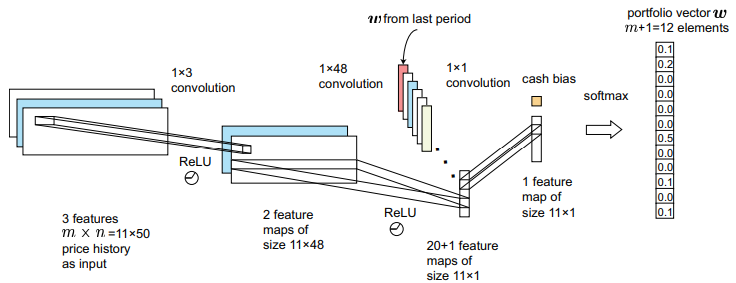
\includegraphics[width=0.9\textwidth]{cnn_eiie_diagram.png}
\end{center}

For the RNN they provide a similar diagram:

\begin{center}
  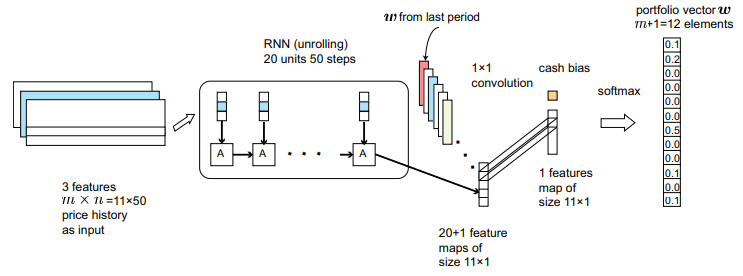
\includegraphics[width=0.9\textwidth]{rnn_eiie_diagram.png}
\end{center}

The three channels in the state matrix on the left are the high, low, and closing price for each asset on each day in the historical sliding window.

The authors claim that this framework beats all of their benchmark strategies in the cryptocurrency market.
The architecture remains essentially the same in our implementation. Due to the use of multiple channels in the state tensor, it makes it easy to
add additional channels for alternative data sources, such as news sentiment.



\section{OLMAR Benchmark Strategy}
\label{olmar_section}
Online Portoflio Selection with Moving Average Reversion (OLMAR), introduced in \cite{olmar_paper}, is used by both \cite{rl_augmented_states} and \cite{drl_framework} as a benchmark strating strategy.
Our codebase includes both custom and library implementations of OLMAR; we provide a brief description of the method here.

Consider a universe of $m$ tradeable assets (and no risk-free asset).
Let $$\Delta_m = \left\{b_t \in \R^m \:|\: b_{t,i} \geq 0 \:\forall i, \sum_{i=1}^m b_{t,i} = 1\right\}$$ be the space of possible portfolios, which is a simplex.
Let $p_t \in \R^{m}$ be the price at time $t$, and and let $x_t \in \R^m$ be the price-relative vector for time $t$, computed as
$x_{t,i} = p_{t,i} / p_{t-1,i}$ for all $i$; that is, $x_t$ is the element-wise division of $p_t$ by $p_{t-1}$.
The goal of the algorithm is to produce a good portfolio $b_{t+1}$ given $p_t, p_{t-1}, ... p_{t-w+1}$ (that is, historical stock prices over a lookback of period $w$).

If we believe that the price of an asset is mean-reverting, then a good prediction for the next price-relative vector $\tilde x_{t+1}$ is
\begin{align*}
  \tilde x_{t+1} = \frac{\mathop{\mathrm{MA}}_t(x)}{p_t} = \frac{1}{w}\left(\frac{p_t}{p_t} + \frac{p_{t-1}}{p_t} + \cdots + \frac{p_{t-w+1}}{p_t}\right)
\end{align*}
To obtain a good return over the next time period, we want $b_{t+1} \cdot \tilde x_{t+1}$ to be high.
However, to keep transaction costs down, we do not want to be too far away from the previous portfolio $b_t$.
Therefore, we formula the optimization problem:
\begin{align*}
  b_{t+1} = \mathop{\mathrm{arg\:min}}_{b \in \Delta_m} \frac{1}{2}\|b - b_t\| \:\:\text{such that}\:\: b \cdot \tilde{x}_{t+1} \geq \epsilon
\end{align*}
for some positive threshold value $\epsilon$. This optimization problem can be solved numerically using standard constrained solvers.

Alternatively, the authors present the following solution: if we ignore the non-negativity constraint, then the solution is
\begin{align*}
  b_{t+1} = b_t + \lambda_{t+1}(\tilde x_{t+1} - \bar x_{t+1} \mathbb{1}) && \bar x_{t+1} = \frac{\mathbb{1} \cdot \tilde x_{t+1}}{m} && \lambda_{t+1} = \max\left\{0, \frac{\epsilon - b_t \cdot \tilde x_{t+1}}{\|\tilde x_{t+1} - \bar x_{t+1} \mathbb{1}\|^2}\right\}
\end{align*}
To enforce the non-negativity constraint, we can project this solution back into the simplex $\Delta_m$.


\section{WMAMR Benchmark Strategy}
Weighted Moving Average Mean Reversion, introduced in \cite{wmamr_paper}, is another trading strategy benchmark used by \cite{rl_augmented_states}.
It is a relatively simple modification to OLMAR, so we will not restate the content of Section \ref{olmar_section}.

The definitions of all terms remain the same. Define the $\epsilon$-insensitive loss function
\begin{align*}
  l_{1,\epsilon}(b, \tilde x_{t+1}) = \begin{cases}
    0 & b \cdot \tilde x_{t+1} \leq \epsilon \\
    b \cdot \tilde x_{t+1} - \epsilon & \text{otherwise}
  \end{cases}
\end{align*}
The authors formula the optimization problem as
\begin{align*}
  b_{t+1} = \mathop{\mathrm{arg\:min}}_{b \in \Delta_m} \frac{1}{2}\|b - b_t\|^2 \:\:\text{such that}\:\: l_{1,\epsilon}(b, \tilde x_{t+1}) = 0
\end{align*}
As with OLMAR, this optimization problem can be solved numerically.
If we ignore the non-negativity constraint, then an analytic solution is
\begin{align*}
  b_{t+1} = b_t - \tau_t(\tilde x_{t+1} - \bar x_{t+1} \cdot \mathbb{1}) && \tau_t = \max\left\{0, \frac{l_{1,\epsilon}}{\|\tilde x_{t+1} - \bar x_{t+1}\|^2}\right\}
\end{align*}
To recover the non-negativity constraint, we project this solution back into the simplex $\Delta_m$.


